\section{Methods}
\label{sec:methods}

\subsection{Data}
\label{sec:data}

\paragraph{Farm photographs.} We used the poultry faecal image collection of Machuve et al.\ released on Zenodo
(record 4628934, CC BY 4.0)~\cite{machuve2022,machuve2021farm}. It contains 6,812 full-resolution smartphone
photographs taken in Arusha and Kilimanjaro, Tanzania, with official bounding boxes in YOLO format for four classes:
healthy, coccidiosis, salmonella and Newcastle disease. According to the record, the healthy and coccidiosis
photographs were taken on poultry farms, the salmonella photographs from experimentally inoculated birds one week
after inoculation, and the Newcastle photographs from inoculated birds within three days. Each class therefore comes
with its own setting. We downloaded the archives through the Zenodo API and checked each against the MD5 checksum
the publisher lists. Following the dataset, we refer to the disease classes as \emph{coccidiosis-like},
\emph{salmonella-like} and \emph{Newcastle-like}, because no photograph in this collection carries a laboratory
diagnosis of its own dropping.

\paragraph{Lab-confirmed photographs.} The same group released a second, separate collection of 1,255 photographs
from layer, cross-bred and indigenous chickens on farms in the same two regions, each coded to a faecal sample that
the dataset authors tested by polymerase chain reaction (PCR) (Zenodo record 5801834)~\cite{machuve2021pcr}. We call
them PCR-labelled or lab-confirmed photographs. They contain 373 coccidiosis, 347 healthy, 349 salmonella and 186
Newcastle disease photographs. No model in this study was trained, tuned or selected on any of them. We use them only
as an external test set. The release contains 35 pairs of byte-identical files, so it holds 1,220 distinct images.
In 19 of these pairs the two files sit in different classes (16 coccidiosis and healthy, 3 healthy and salmonella),
so at least 19 labels or file placements are wrong. We report results on all 1,255 files, as released, and give the
effect of removing the 38 conflicting files in Section~\ref{sec:res-bench}.

\paragraph{Barn video.} To teach the detector the size droppings have in a fixed pen camera, we took background
frames from two public video collections of broiler houses: the PIO videos (Zenodo record 16686320, CC BY
4.0)~\cite{boniche2025piodata,boniche2026pio} and the NESTLER poultry videos (Zenodo record 15063494, CC BY 4.0)~\cite{nestler2025}. No dropping in these
videos is labelled, and we did not label any.

\subsection{Split}
\label{sec:split}

The 6,809 farm photographs that have labels (three label files are empty) were split 80/10/10 by photograph within
each class, using a fixed seed on the sorted file names, giving 5,451 training, 679 validation and 679 test
photographs. This is the kind of random split earlier work
on this collection reports. The detector and every baseline in Section~\ref{sec:bench} use exactly this split. To
measure leakage, we reduced every photograph to a 256-bit difference hash~\cite{krawetz2013} and recorded, for
each test photograph, the Hamming distance to the closest training photograph.

\subsection{Detector}
\label{sec:detector}

Our detector is YOLO11n~\cite{jocher2024yolo11} with four classes, fine-tuned from COCO weights at 640 pixels with early stopping (patience 20, seed 0) on a local laptop GPU. The Newcastle-like class has about a sixth of the
photographs of the others, so its training photographs are repeated three times, after the split and in the training
set only. Training stopped at epoch 69 and the weights of epoch 49, the best on validation, were kept
(\texttt{dropping4-laptop}). We exported it to ONNX at 320, 416 and 640 pixels. To check that the result does not depend on the machine, we repeated the training on the Veri cloud
platform on one NVIDIA A10G GPU, with batch 32 and a 30-minute limit (20 epochs). That run reached a test mAP50
of 0.854 and mAP50-95 of 0.573, against 0.873 and 0.573 for the local run, so the two are close. All results below
use the local run.

To compare the detector with photograph classifiers, we score a whole photograph with it: the photograph is
letterboxed to 640 pixels, every candidate box keeps its class scores, and each class takes its best score in the
photograph. The photograph's call is the class with the highest score, or \emph{no detection} when no box reaches
0.25, the confidence threshold the deployed pipeline uses.

\subsection{Pen-scale fine-tuning}
\label{sec:pen}

We handle pen frames at $1280\times720$ and assume that a dropping spans 8 to 30 pixels along its longest side there.
This is a design assumption for a ceiling camera over a pen, not a measurement, since no droppings in our pen videos
are labelled. In the farm collection, by contrast, the disease-class boxes cover a median of 12 to 22\% of the
photograph. We built a pen-scale training set by copy-paste
augmentation~\cite{ghiasi2021}: real labelled droppings were cut from the farm photographs along their
official boxes, shrunk to pen size, and pasted onto empty litter in barn video frames. A dropping from a training
photograph is only ever pasted into a training tile, and likewise for validation and test, so the farm split carries
over. Background frames were split \emph{by camera}, never by frame. Five PIO videos and the remaining NESTLER cameras
form the training set, one NESTLER camera the validation set, and three NESTLER cameras plus the PIO video used in our
live demonstration the test set. Frames with birds and equipment and no pasted dropping were kept as negatives. The
model \texttt{dropping4-pen} was fine-tuned from \texttt{dropping4-laptop} on these tiles mixed with the original
farm photographs, for up to 40 epochs (patience 10). It stopped at epoch 38.

We state the limitation plainly: the pen test is synthetic. It measures whether the model finds a real dropping of
pen size on litter and cameras it has never seen, not field accuracy on naturally occurring droppings.

\subsection{Baselines}
\label{sec:bench}

Published results on this collection come from different splits, image sizes and protocols, so we retrained the
classifiers earlier work used instead of quoting their numbers. MobileNetV2~\cite{sandler2018} is the model
Machuve et al.\ recommended for deployment~\cite{machuve2022}, EfficientNet-B0~\cite{tan2019} is the
classifier stage of a recent YOLO11 and EfficientNet-B0 pipeline~\cite{dhungana2025}. Each was
initialised from ImageNet weights and trained on the same 5,451 training photographs, resized to $224\times224$
without keeping the aspect ratio (as in the 224-pixel copy of the collection most earlier work used), with AdamW and a
one-cycle learning rate schedule. MobileNetV2 was trained for 20 epochs and EfficientNet-B0 for 8, both with one seed,
because of the compute time available to us. Augmentation
was random crops, horizontal and vertical flips, and small brightness and contrast changes. We did not change hue,
because colour is the main visual sign of disease. The epoch with the best validation accuracy was kept. Both passed 98\% validation accuracy within four epochs, so the shorter EfficientNet-B0 run is unlikely to change
the comparison, but one seed cannot measure run-to-run variation.

\subsection{Evaluation}
\label{sec:eval}

All models are scored on the same 679 farm test photographs and the same 1,255 lab-confirmed photographs. We report
accuracy, per-class recall and macro-F1. Proportions carry 95\% Wilson score intervals~\cite{wilson1927}, which
behave well near 0 and 1. For the detector we also report a risk-coverage curve~\cite{geifman2017}, the
accuracy of the answers when the model only answers above a confidence threshold, and a reliability diagram with the
expected calibration error over ten equal-width bins~\cite{guo2017}.

\subsection{Appearance grades for the lab-confirmed photographs}
\label{sec:grades}

PCR says whether a pathogen is in the sample, not how the dropping looks. To ask whether the models fail on
droppings that look normal, we graded every one of the 1,255 lab-confirmed photographs for appearance. A written
rubric scores six visual variables 0, 1 or 2, or leaves them empty when the photograph does not show them: form,
the white urate cap, colour, blood, mucus or foam, and undigested feed. These are the signs used in clinical checks
of droppings. The grade is computed, never chosen, as $\max(1, 10 - p)$ where $p$ is the sum of the six scores with
blood counted twice, so every lost point has a named reason. Grades 9 and 10 mean the dropping looks normal.

The raters were three AI vision models, not people: Claude Opus, Claude Sonnet and Claude Haiku, each run with
the same written instructions and no shared context. Each photograph got a random identifier and was re-encoded
at 768 pixels with no metadata, and the key linking identifiers to file names and PCR classes stayed outside the
raters' folder until grading ended. Each rater saw the photographs in its own random order. 126 photographs (10\%)
were shown a second time under a new identifier to measure each rater's agreement with itself. The released
sub-score for a photograph is the median of the raters who could judge it, needing at least two, and its grade is
recomputed from those medians. We report Krippendorff's alpha for ordinal data across the three
raters~\cite{hayes2007} and quadratic weighted kappa for each pair and for each rater against itself~\cite{cohen1968}.

\subsection{Deployment on QNX}
\label{sec:qnx}

The deployed system runs on a Raspberry Pi 5 with a Camera Module 3 under QNX 8.0, a microkernel real-time operating
system~\cite{qnx8sysarch}. The pipeline is split into separate processes (sections), each with its own memory and a
fixed real-time priority: camera capture in C, a still-spot finder that flags new objects that appeared and stayed
still, the detector, an explanation step, and links to the dashboard and a wrist-worn display. Full frames stay in a
shared-memory ring of four slots, and sections exchange only small messages through QNX native message passing. A
supervisor restarts any section that exits. On the Pi the detector is the close-up model, run on a full-resolution
patch around each candidate from the spot finder, not the pen model. At pen scale the close-up model can score white
birds as salmonella, so the explanation step dismisses a candidate unless its box lies on the spot, has the size of a
dropping, is not white, is not lighter than the floor around it, and scores at least 0.6. Inference uses ONNX Runtime~\cite{onnxruntime} 1.24.4 from the QNX
open-source package repository, called from a small C bridge because the repository's Python binding does not load on
QNX (Section~\ref{sec:discussion}). We report the detector's inference time on the Pi with four threads, without image
decoding or post-processing.

Alerts reach people in two ways. A wrist-worn display polls the dashboard and shows each pen's state. A separate
messaging service sends pen alerts to the farmer over iMessage through the Photon platform and answers follow-up
questions in plain language with a large language model (DeepSeek). Each alert states what the camera recorded, the
model's closest match with its score, and that it is not a laboratory test. The service never tells the farmer to
treat or cull birds. It contacts a veterinarian only after the farmer clearly agrees, and that decision is made by
tested rules in the application code, not by the language model. We describe this service for completeness and do not
evaluate it here. Figures~\ref{fig:hardware} and~\ref{fig:interfaces} show the hardware and the three interfaces.

\begin{figure*}[t]
\centering
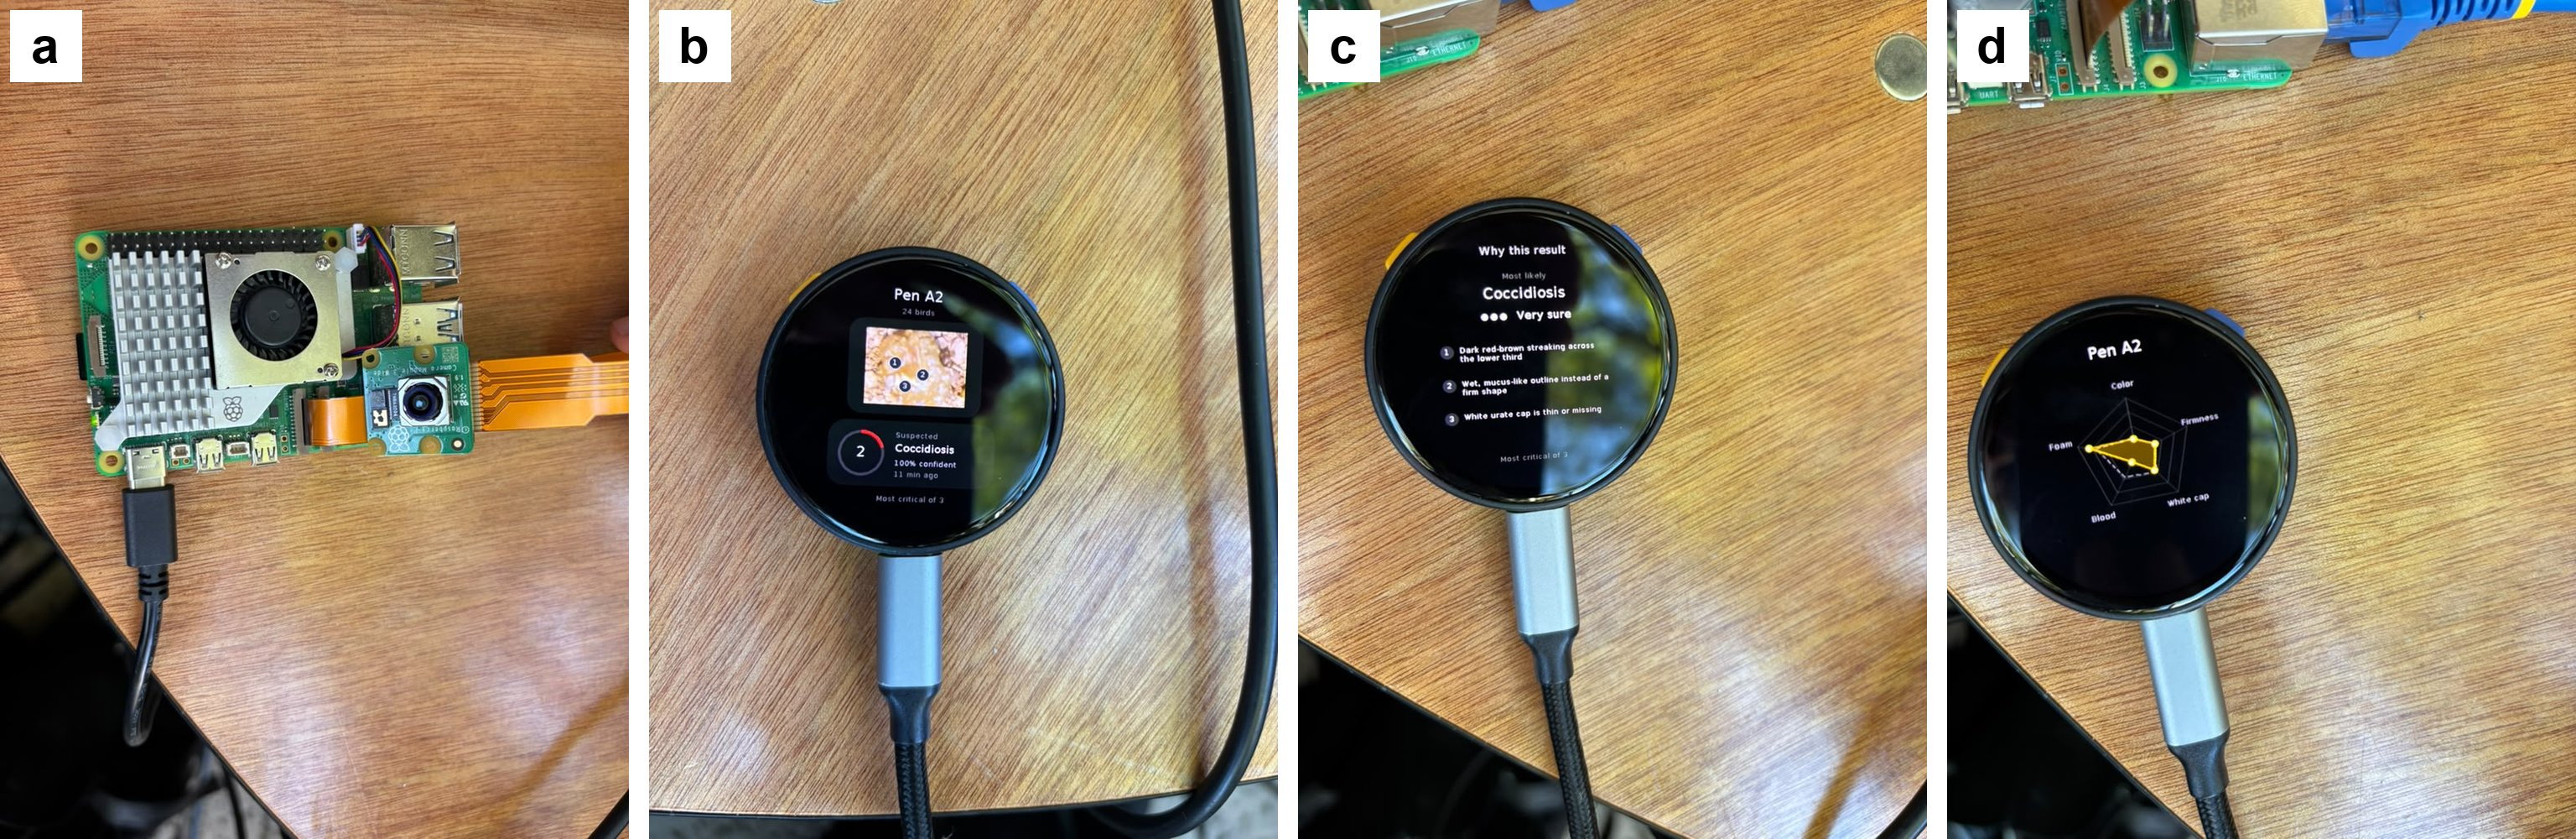
\includegraphics[width=\textwidth]{figures/system_hardware.jpg}
\caption{The deployed hardware. (a) Raspberry Pi 5 running QNX 8.0 with a Camera Module 3 on its ribbon cable and an
active cooler. (b to d) The wrist-worn display (M5Stack StopWatch) on its charging cable, showing a pen's newest
specimen with its photograph and numbered evidence markers (b), the evidence in words (c), and the pen's five
appearance checks against the barn average (d). The display is shown with the dashboard's demonstration data, not a
field reading.}
\label{fig:hardware}
\end{figure*}

\begin{figure*}[t]
\centering
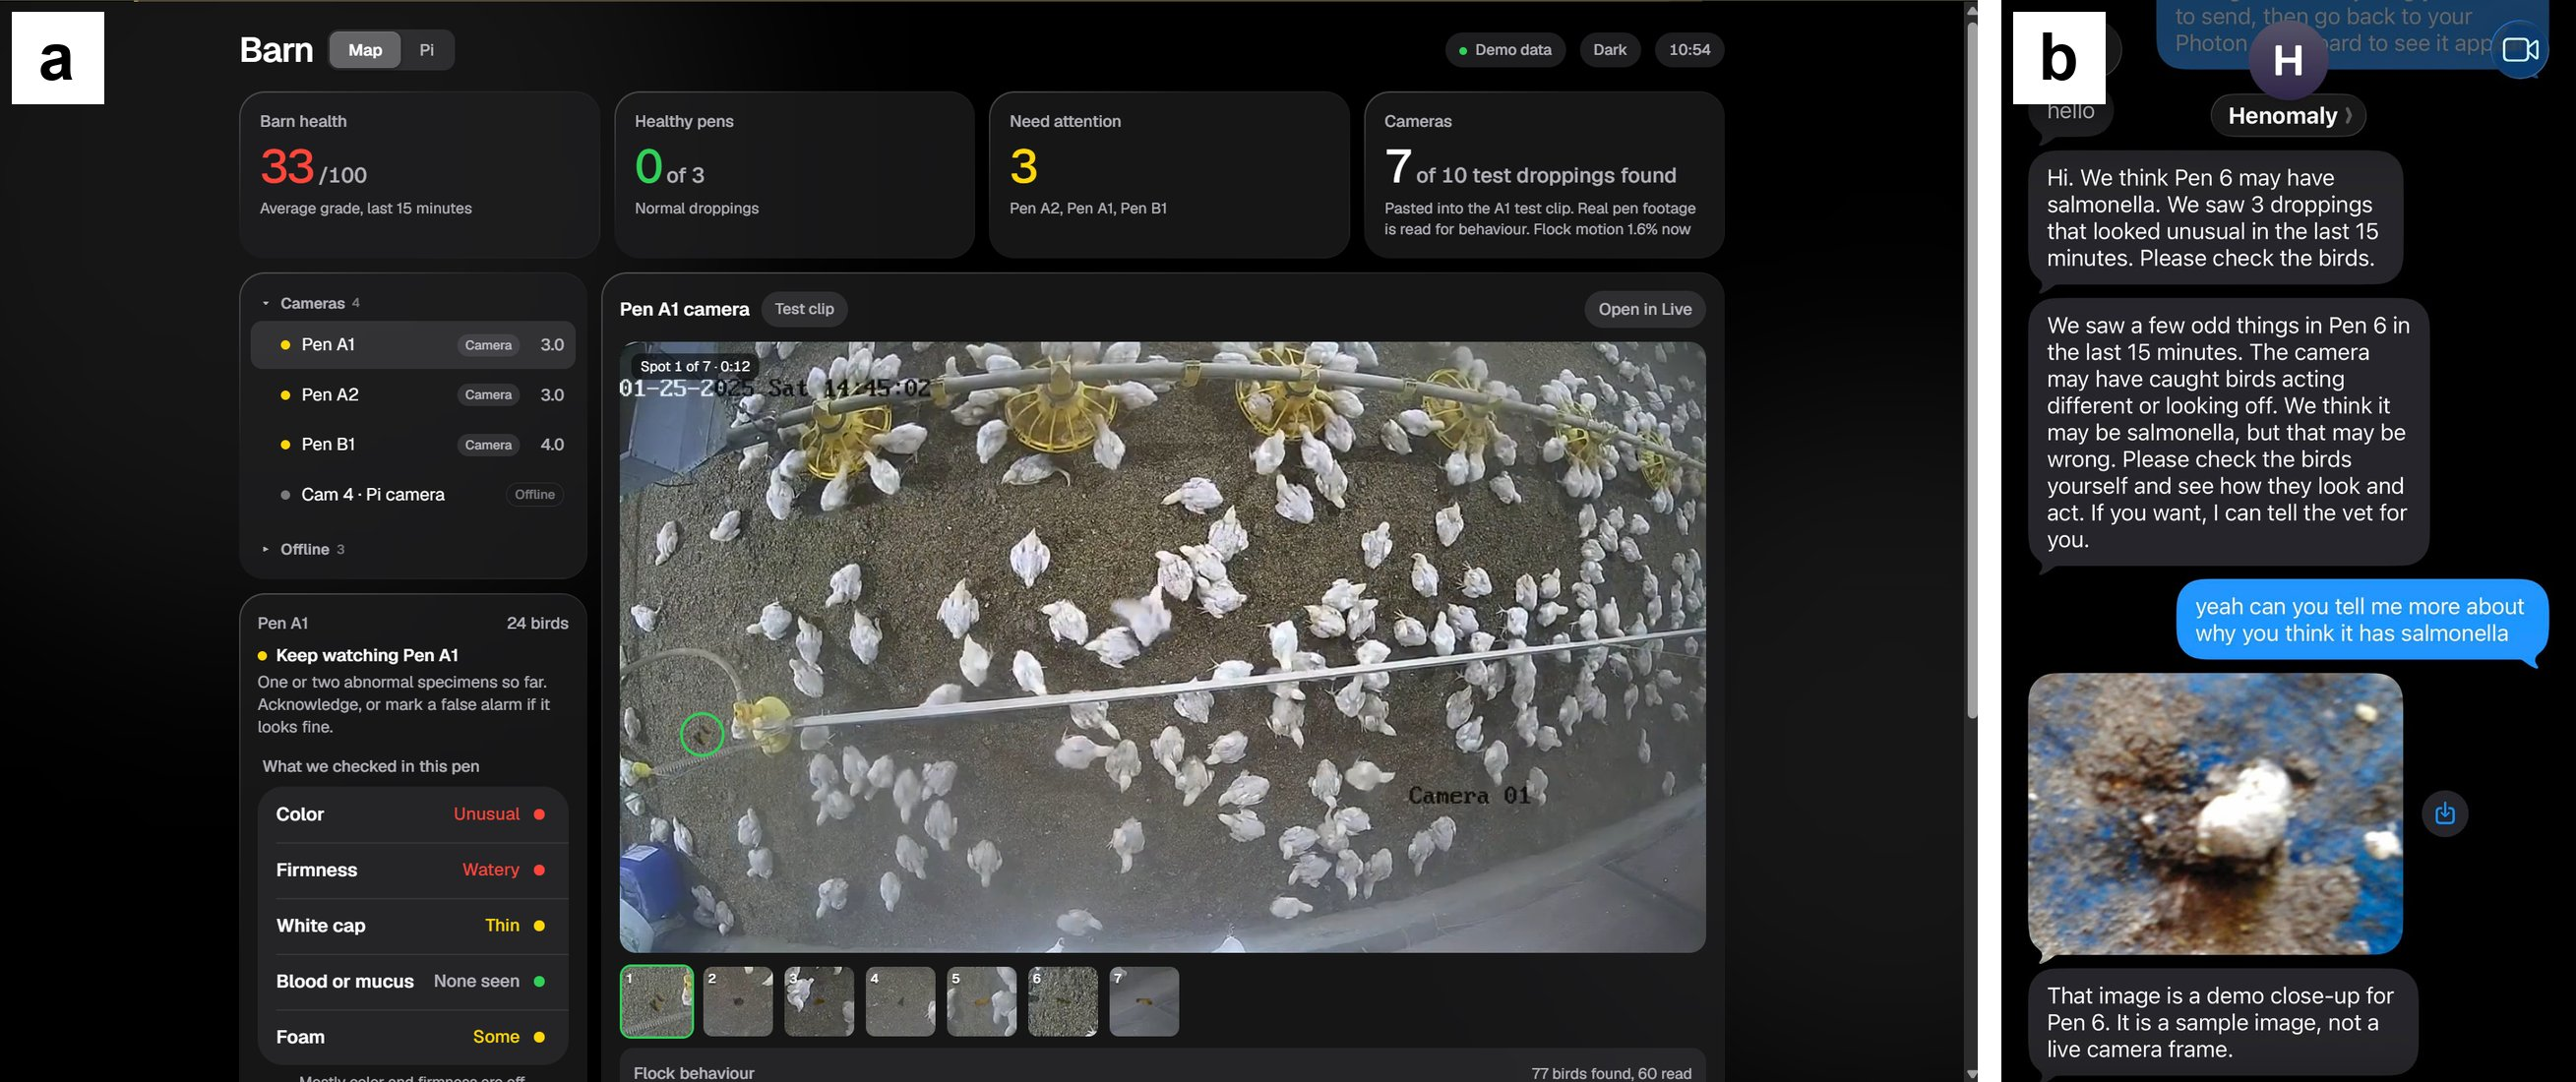
\includegraphics[width=\textwidth]{figures/system_interfaces.jpg}
\caption{The two other interfaces. (a) The dashboard with the held-out Pen A1 test clip, in which test droppings were
pasted at known times. A green ring marks a flagged spot and the strip below lists the seven spots found. Pen
readings on the dashboard are demonstration data, as its header states. (b) The farmer messaging service in a test
conversation. The attached photograph is a sample image, as the agent itself says, not a live camera frame.}
\label{fig:interfaces}
\end{figure*}
